\chapter{CoNtRoL Simulations Web Application}
\label{ch:web-app}

\textit{ Here we will present the open-source Web application developed for easing work involving chemical reaction networks, hopefully for students and researchers one day. It can be used for obtaining numerical analysis of chemical reaction networks, as well as plotting species against time, one another and even the graph of a network. We'll present the technologies used throughout the project, how to run it locally and a couple of usage examples involving what we've presented in the previous chapters. A lot of the heavy lifting was done by these libraries \footcite{10.1093/bioinformatics/btac730, xu2023SbmlDiagrams, medley2018tellurium, choi2018Tellurium}. I've also had the opportunity of contributing a commit or two to \href{https://github.com/sys-bio/tellurium}{Tellurium}, one of core libraries, during the making of this app.}

\subsection{Overview of the technologies}
The website is a back-end application built in \textbf{Python}, a programming language known for its use in basically every single science, including natural sciences so it's a no-brainer when in comes to plotting.

The web server is built using \textbf{Flask}, a lightweight web app framework and the webpages served are server-side rendered by Flask's template engine depedency - \textbf{Jinja}.
\\
The crux of the functionality is aided by the Python library \textbf{Tellurium}\footcite{choi2018Tellurium,medley2018tellurium}; which is, as their docs say; "A Python Environment for Reproducible Dynamical Modeling of Biological Networks". It uses a subset of the Systems Biology Markup Language ( \textbf{SBML})\footcite{xu2023SbmlDiagrams,bornstein2008Libsbml, 10.1093/bioinformatics/btac730} called \textbf{Antimony} which can be used in this app to create a Chemical Reaction Network, as well as the friendlier selects form. So the bits doing the magic are the calls to \verb|road_runner.loada()| which are used to \textbf{\textit{load}}    \textbf{a}ntimony code into the model.
the \verb|road_runner.simulate()| function is then used for running and obtaining sumulation data, followed by \verb|road_runner.plot()|, which in turn calls a \verb|matplotlib| headless backend for writing the plotted results to a file.

\subsection{Running it}
As explained in the \verb|README| of \href{https://github.com/viktorashi/Open-CoNtRol}{the project}, installing and running locally is a bit more tedious and highly depends on which opperating system you're running, but the general overview goes, kind-of like this:. \\\\

\tikz\draw[black,fill=black] (0,0) circle (.5ex); clone the project

\begin{lstlisting}[language=bash]
    git clone https://github.com/viktorashi/Open-CoNtRol.git
\end{lstlisting}

\tikz\draw[black,fill=black] (0,0) circle (.5ex); \textbf{c}hange \textbf{d}irectory into it.

\begin{lstlisting}[language=bash]
    cd Open-CoNtRol
\end{lstlisting}

\tikz\draw[black,fill=black] (0,0) circle (.5ex); (optionally) install \href{https://virtualenvwrapper.readthedocs.io/en/latest/}{virtualenvwrapper} (which I reccomend) and create a \textbf{virtual environment}

\begin{lstlisting}[language=bash]
    mkvirtualenv control #or whatever you want to name it
\end{lstlisting}

Now here comes the part depending on your OS: You need to install \href{https://pygraphviz.github.io}{PyGraphviz}, which is essential to plotting the Graph view of networks, but it uses a C/C++ back-end so it's not as easy a simple \verb|pip install|

\tikz\draw[black,fill=black] (0,0) circle (.5ex); On Linux:
\begin{lstlisting}[language=bash]
    sudo apt-get install graphviz graphviz-dev
    pip install pygraphviz
\end{lstlisting}

\tikz\draw[black,fill=black] (0,0) circle (.5ex); On macOS:
\begin{lstlisting}[language=bash]
    #first install \href{https://brew.sh}{Homebrew}
    /bin/bash -c "$(curl -fsSL https://raw.githubusercontent.com/Homebrew/install/HEAD/install.sh)"
    brew install graphviz
    pip install pygraphviz
\end{lstlisting}

\tikz\draw[black,fill=black] (0,0) circle (.5ex); And if that doesn't work (usually because of newer macOS versions), change the third part of the installation like so:

\begin{lstlisting}[language=bash]
pip install --config-settings="--global-option=build_ext" \
            --config-settings="--global-option=-I$(brew --prefix graphviz)/include/" \
            --config-settings="--global-option=-L$(brew --prefix graphviz)/lib/" \
            pygraphviz
\end{lstlisting}

\tikz\draw[black,fill=black] (0,0) circle (.5ex); For Windows, I just use \href{https://learn.microsoft.com/en-us/windows/wsl/install}{WSL}:

Now this part is the same no matter which OS you use

\tikz\draw[black,fill=black] (0,0) circle (.5ex); install the rest of the requirements

\begin{lstlisting}[language=bash]
    pip install -r requirements.txt
\end{lstlisting}

\tikz\draw[black,fill=black] (0,0) circle (.5ex); Now I suggest you just
\begin{lstlisting}[language=bash]
    flask run
\end{lstlisting}

\tikz\draw[black,fill=black] (0,0) circle (.5ex); Orrr
\begin{lstlisting}[language=bash]
    python -m flask run
\end{lstlisting}

\tikz\draw[black,fill=black] (0,0) circle (.5ex);
But if that doesn't work, give the \verb|run_script.sh| execute permissions

\begin{lstlisting}[language=bash]
    chmod +x ./run_script.sh
\end{lstlisting}

\tikz\draw[black,fill=black] (0,0) circle (.5ex);
and give it a shot

\begin{lstlisting}[language=bash]
    ./run_script.sh
\end{lstlisting}

Among the wall of output will also be the line showing the address your server is located at, for example:
\verb|* Running on http://127.0.0.1:5000|, address at which you'll be greeted with this screen

\[
	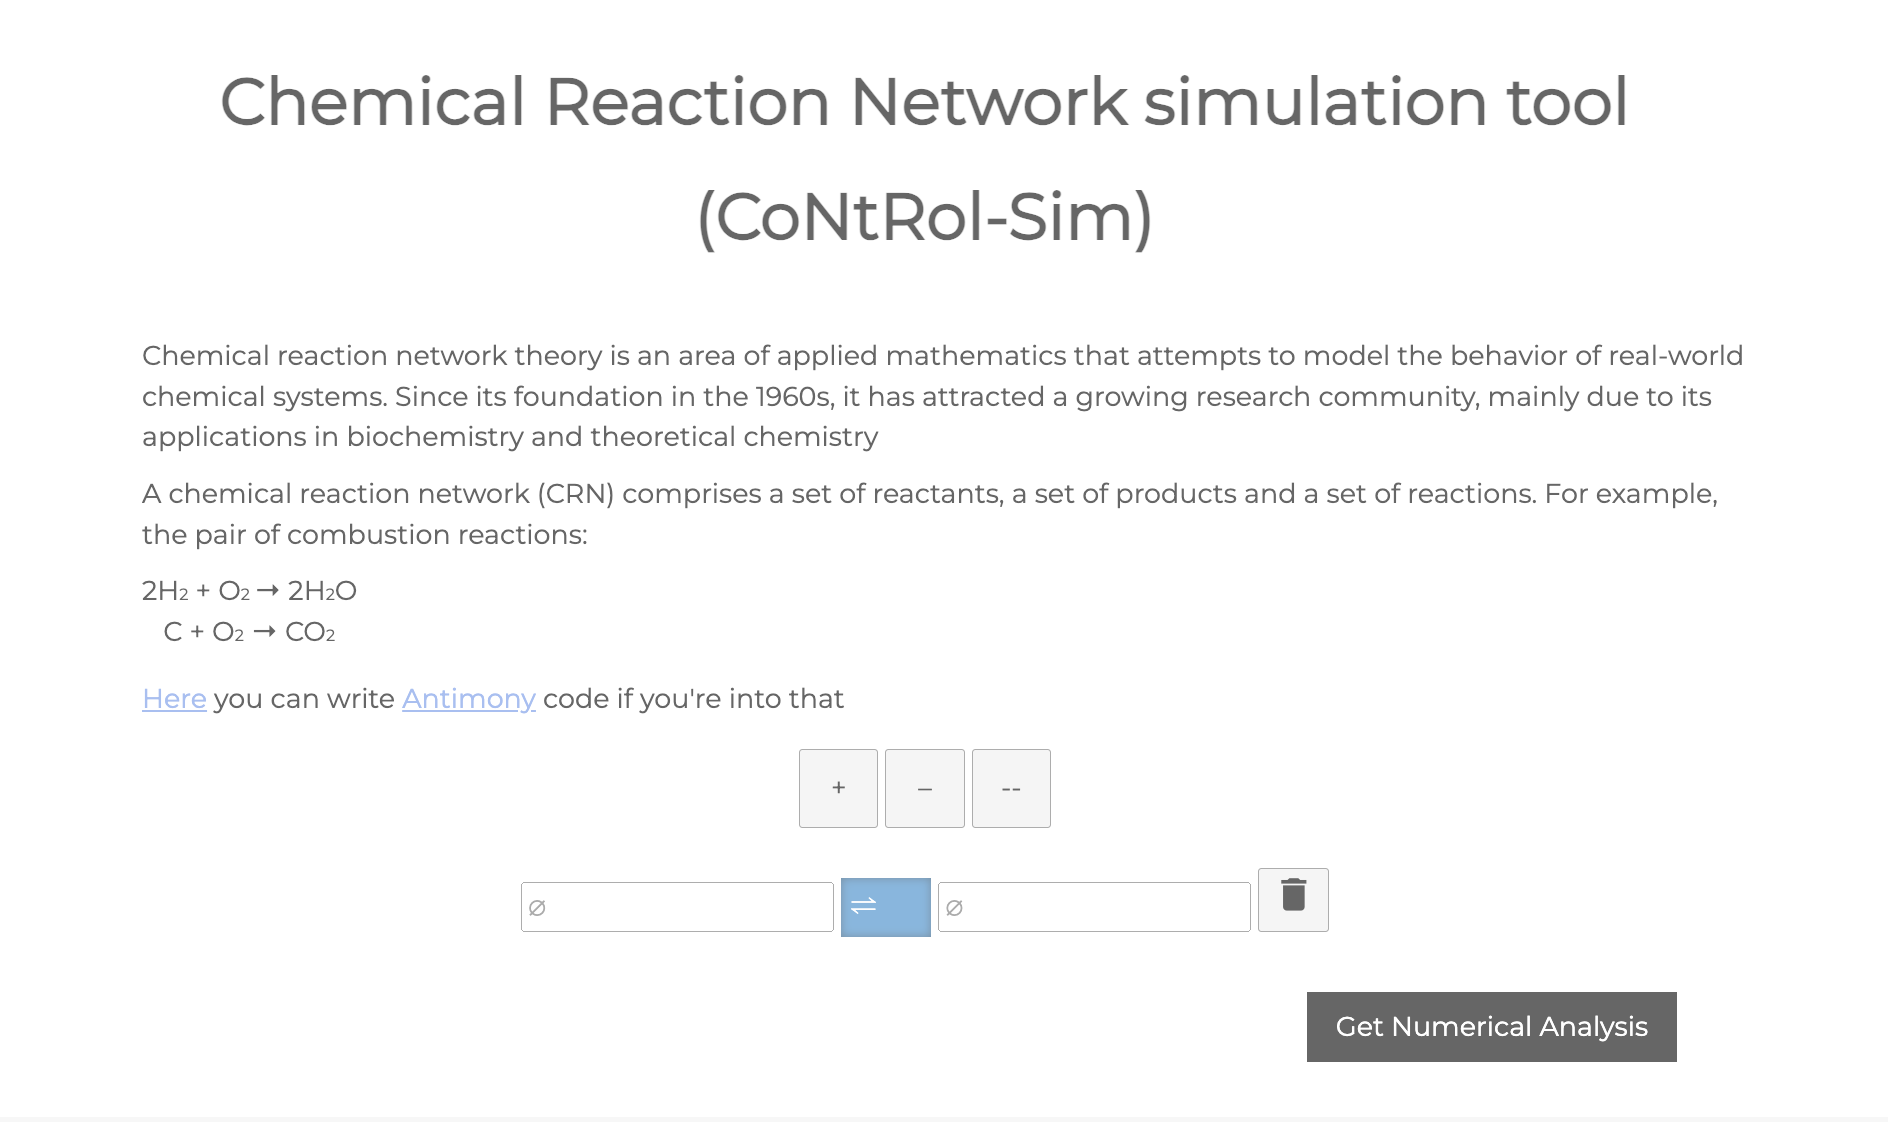
\includegraphics[width=13cm]{app_photos/control_home_screen.png}\\
\]

To start, you can either start typing equations inside those pre-aligned fields like so:

\[
	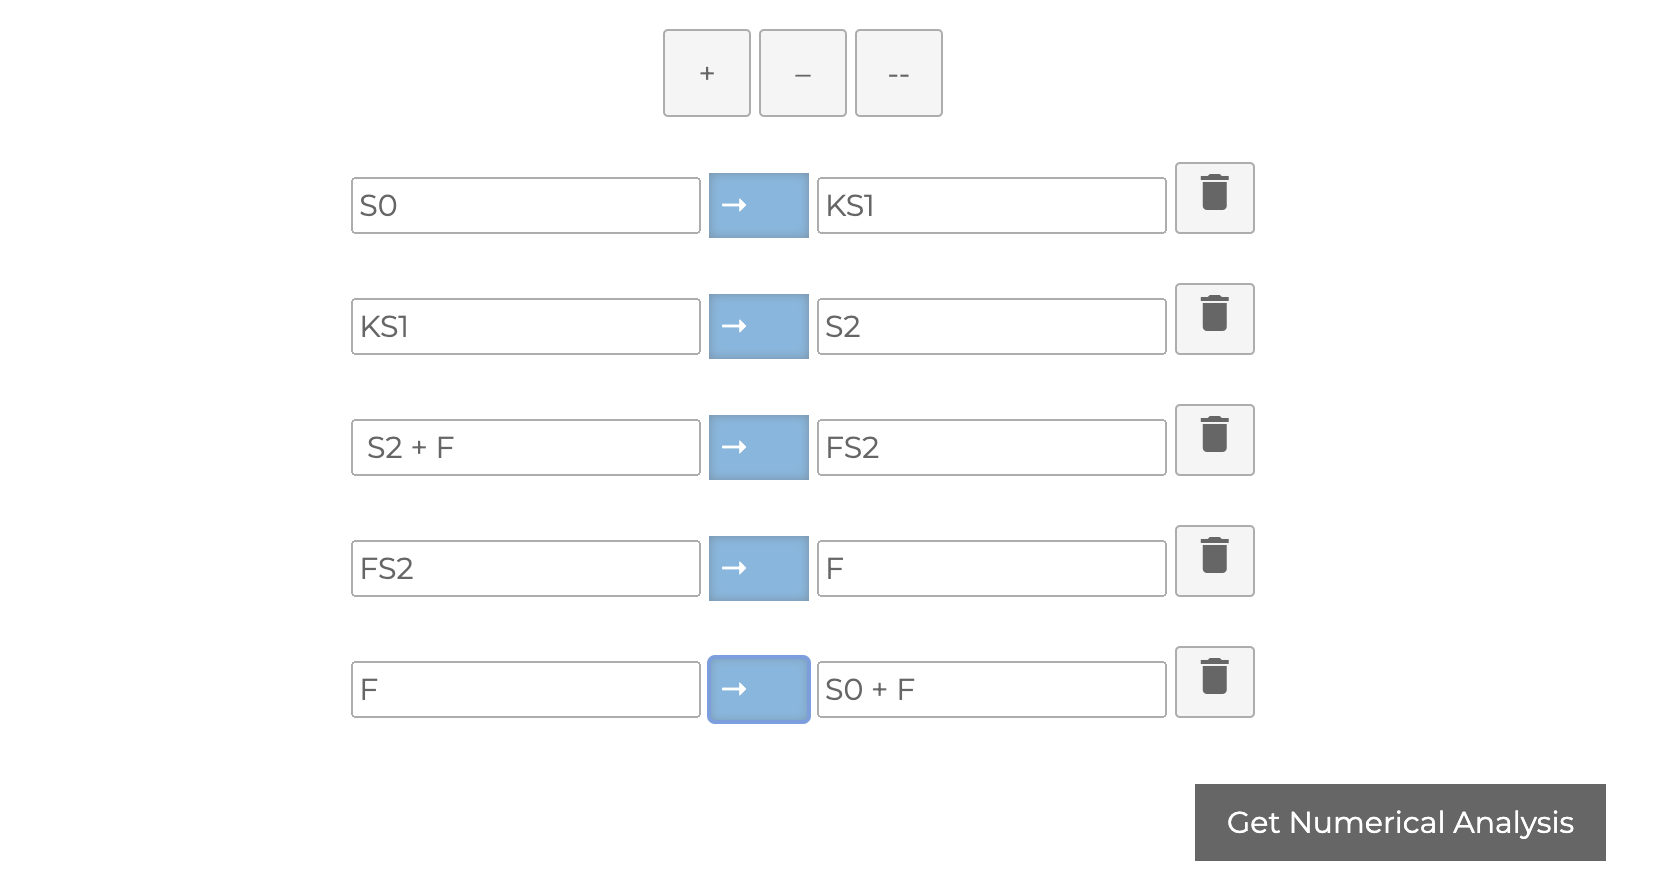
\includegraphics[width=13cm]{app_photos/creca-prima-data-cand-am-scris-asta.png}\\
\]

or put the equations you're analysing:

\begin{lstlisting}
S0 -> KS1
KS1 -> S2
S2 + F -> FS2
FS2 -> F
F -> S0 + F
\end{lstlisting}

right into the \verb|textfield| that pops up when clicking "Write CRN".

\[
	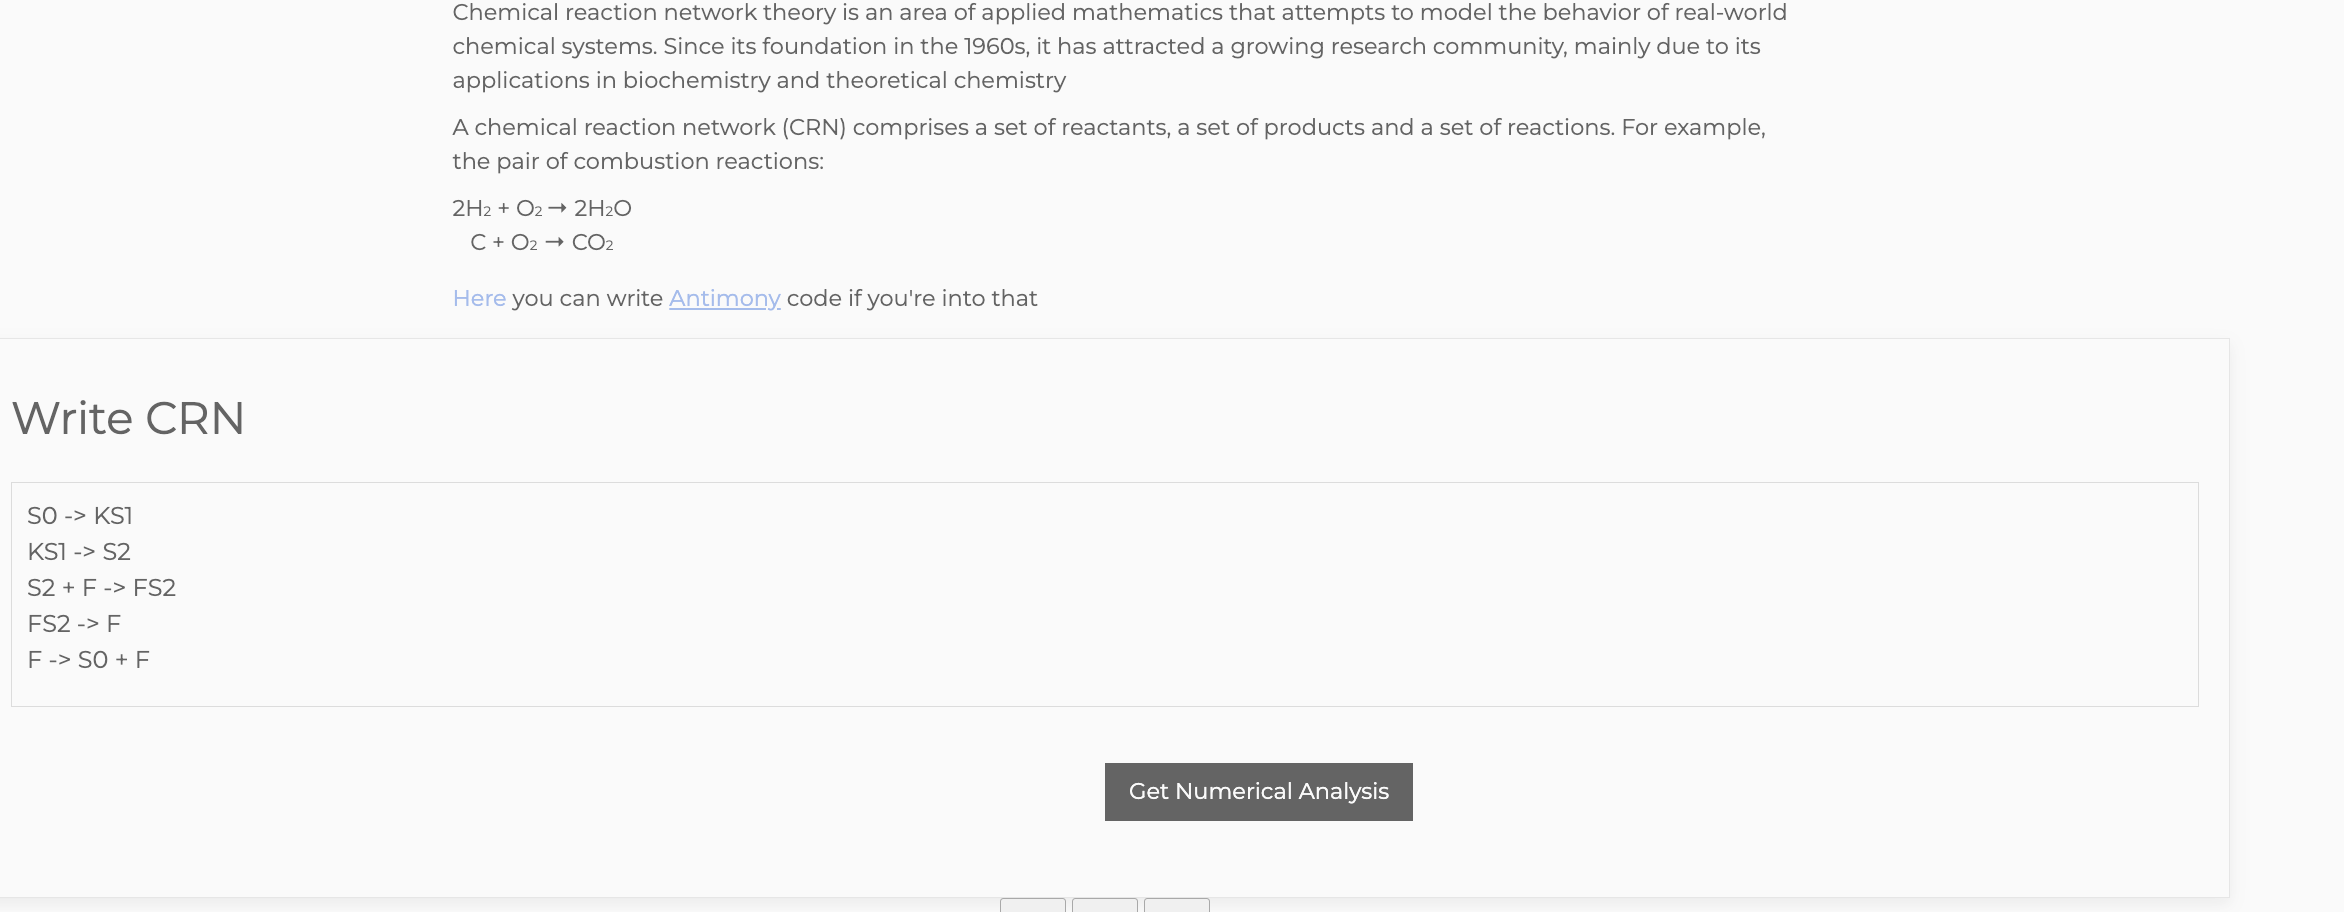
\includegraphics[width=13cm]{app_photos/antimony_area.png}\\
\]

both of these options / paths yield the same numerical analysis results:

\[
	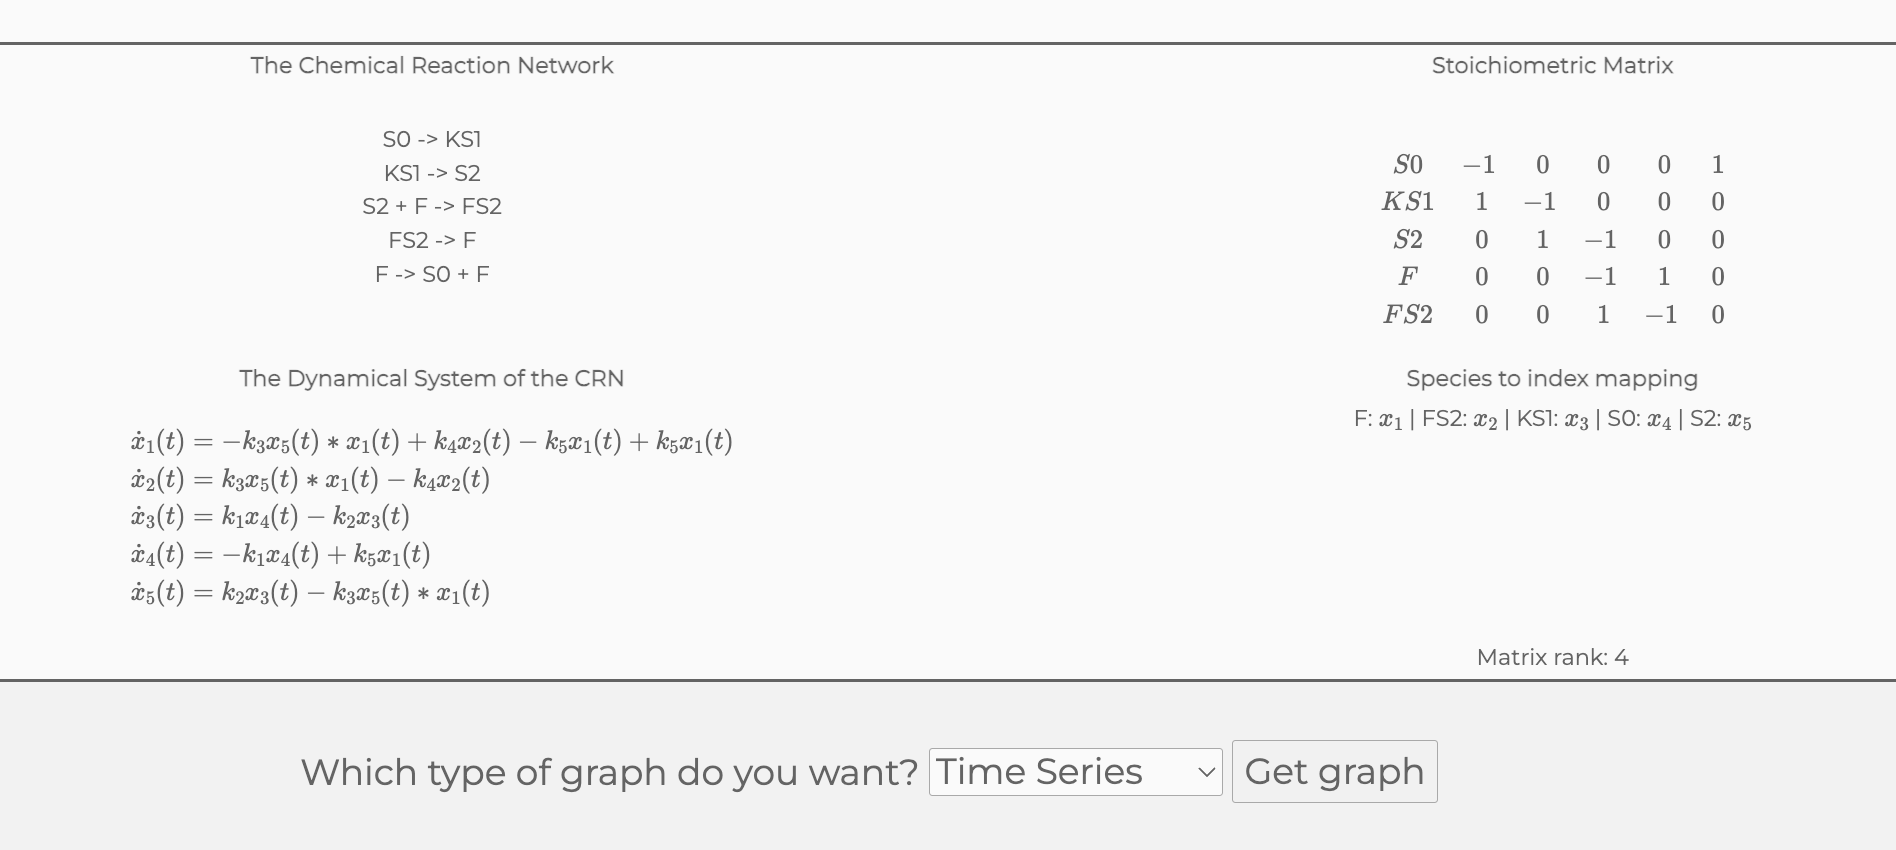
\includegraphics[width=13cm]{app_photos/numerical_analysis.png}\\
\]

from here, one can choose from a selection of graphs they can represent given this system, the default one being the time series representation:

\[
	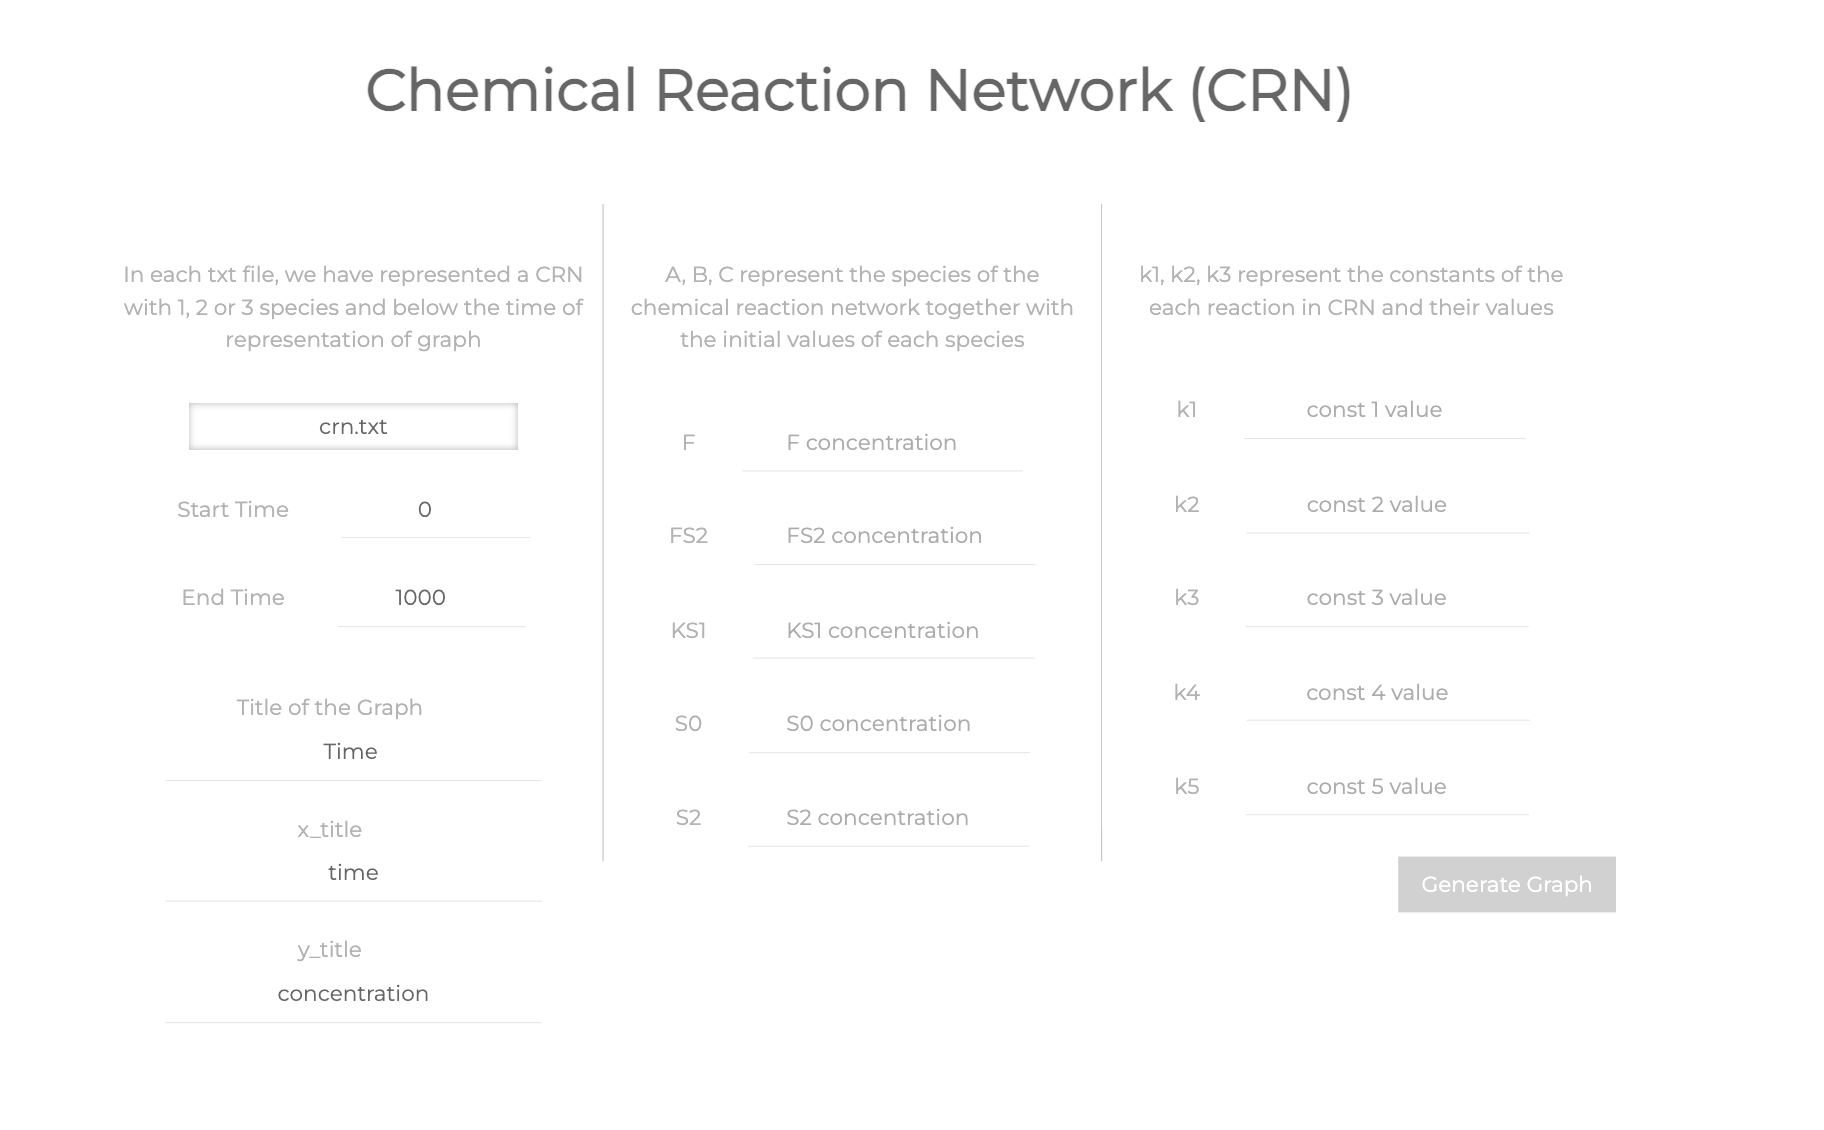
\includegraphics[width=13cm]{app_photos/tsr-input.png}\\
\]

from which we fill out the initial values of the concentrations for each species as, well as the reaction rates. As you can see, we've found oscillations for network \ref{network3_irr_ss} \label{last_system_init_cond}
\begin{lstlisting}
    F = 0.874108
    FS2 = 7.620157734
    KS1 = 7.620157734
    S0 = 7.270157734
    S2 = 0.6

    k1 = 0.1329759342
    k2 = 0.1329759342
    k3 = 2
    k4 = 0.1329759342
    k5 = 1
\end{lstlisting}

outcomes the graph:

\[
	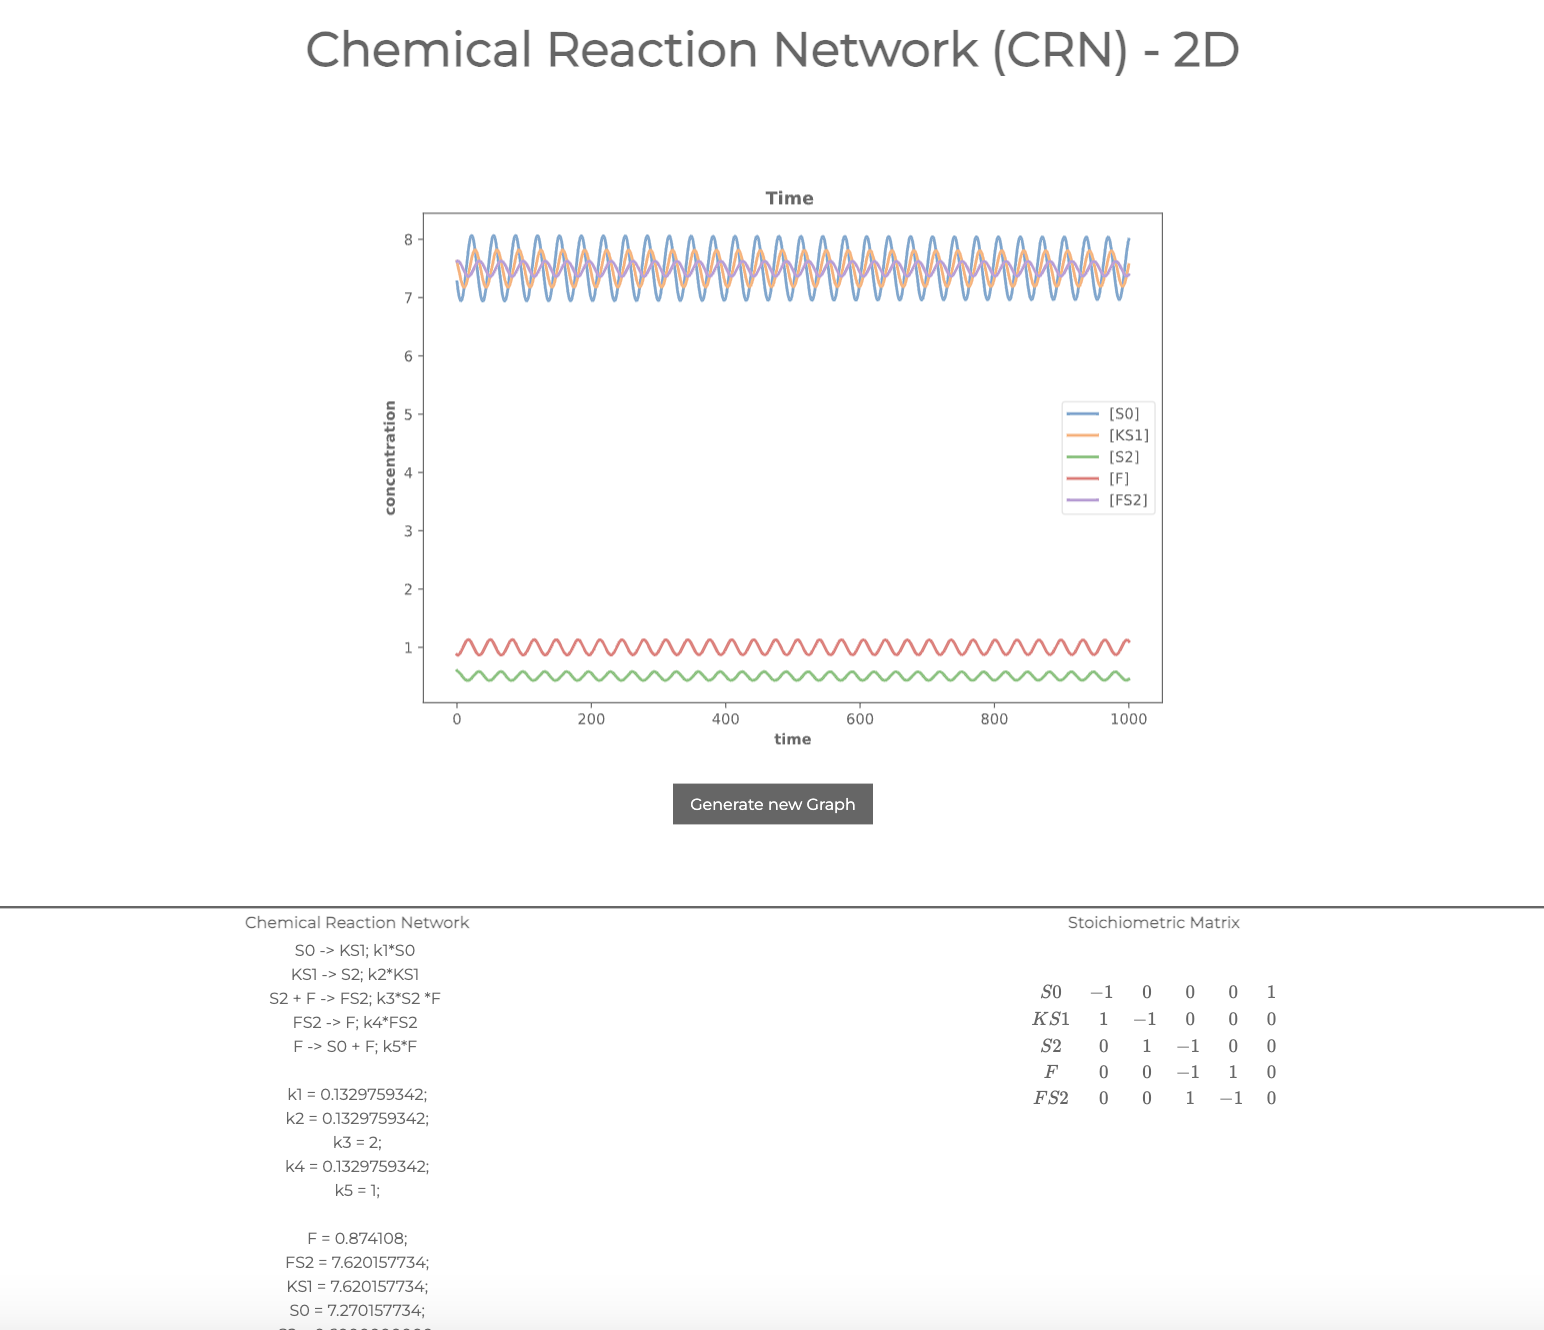
\includegraphics[width=13cm]{app_photos/a-graph-indeed.png}\\
\].

\subsection{The bottom line}

So this is how the workflow of the app typically goes. \\
$
\begin{WithArrows} & \textit{write out your system} \rightarrow \textit{get numerical analysis} \rightarrow \textit{choose your desired graph} \Arrow{\textit{fill out data values}}  \\
	& \hfill \textbf{Voilà}
\end{WithArrows}
$

Some other types of graphs are:

The DSR Graph from \href{https://github.com/sys-bio/roadrunner}{libroadrunner}, whose Python API could only display them inside \href{https://jupyter.org}{notebooks}, but a few \href{https://github.com/sys-bio/tellurium/pull/597}{tweaks} of mine, is now able to also display to a file and hence, use in thi web-app.

\[
	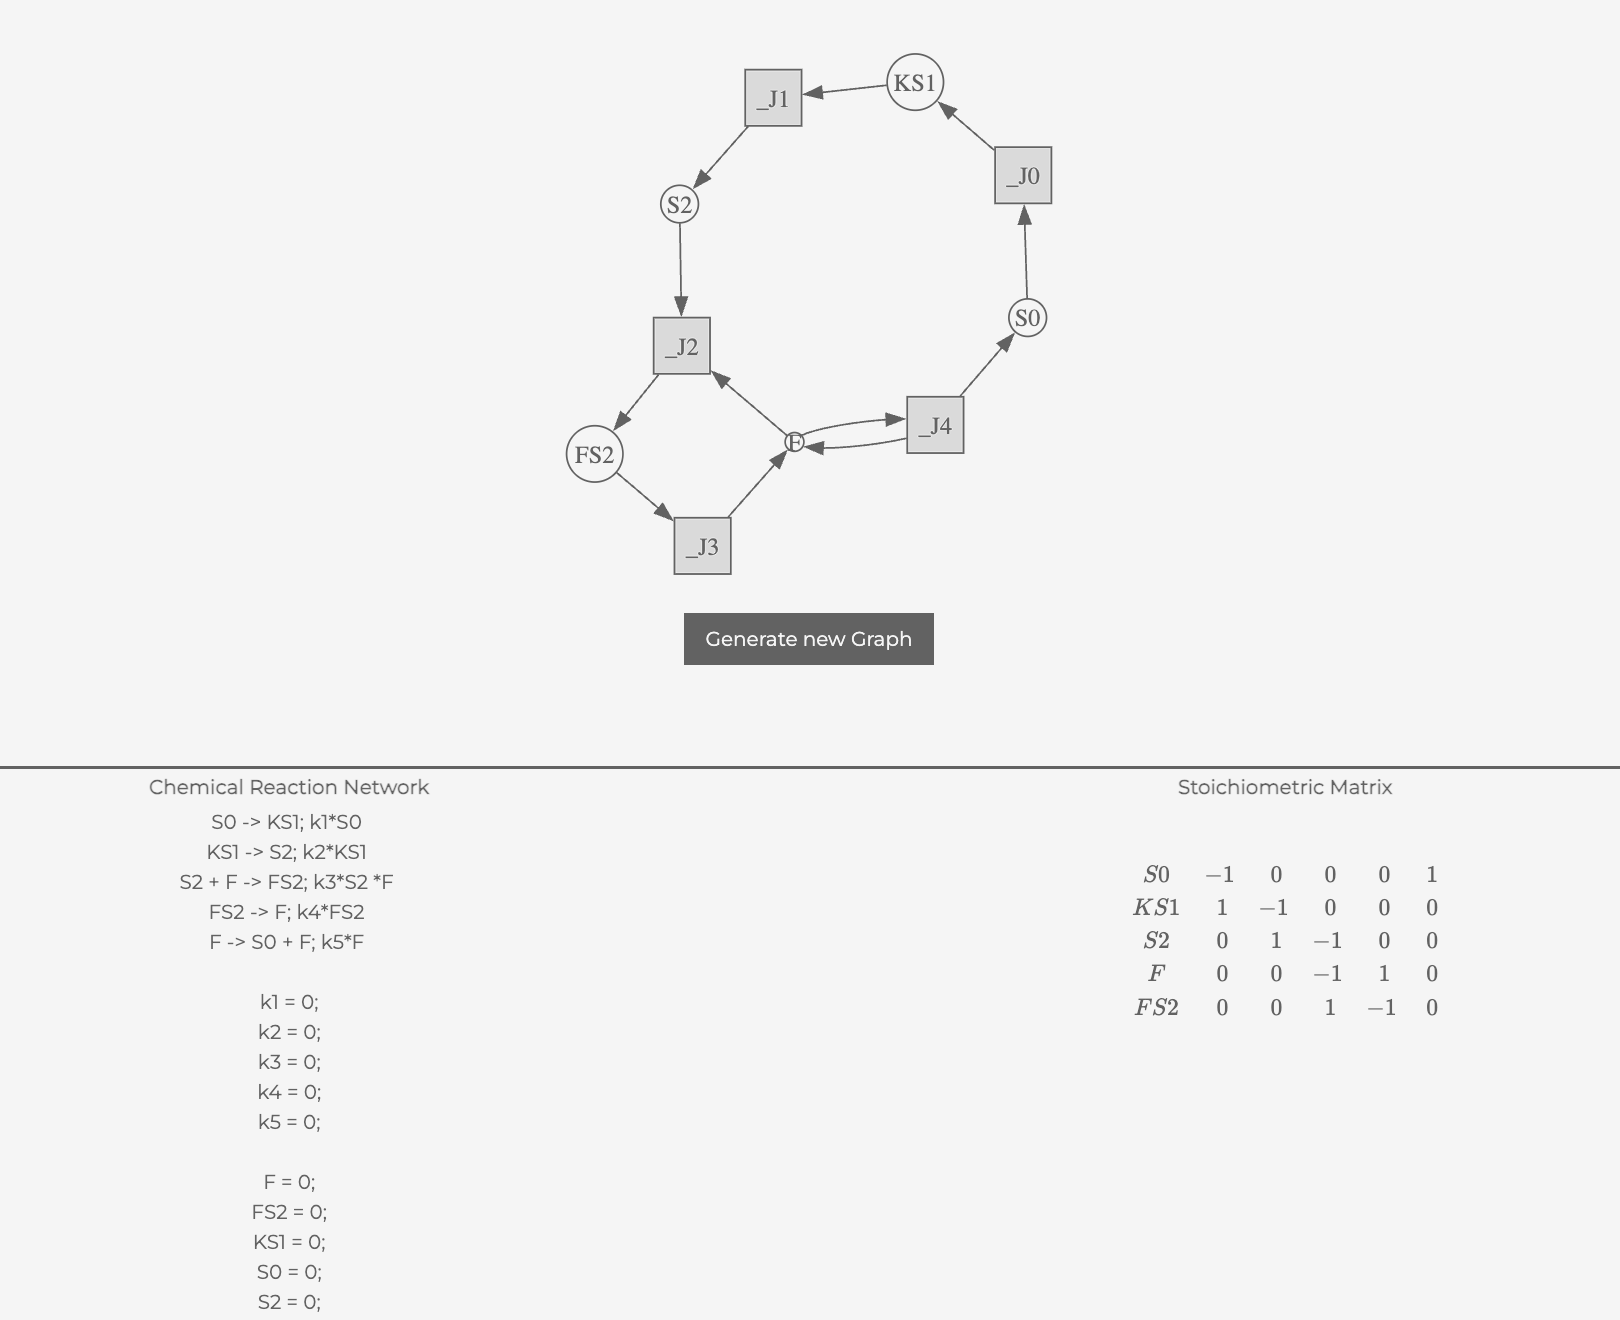
\includegraphics[width=13cm]{app_photos/dsr-graph.png}\\
\].

Another important feat was being able to plot multiple species against one-another.

\[
	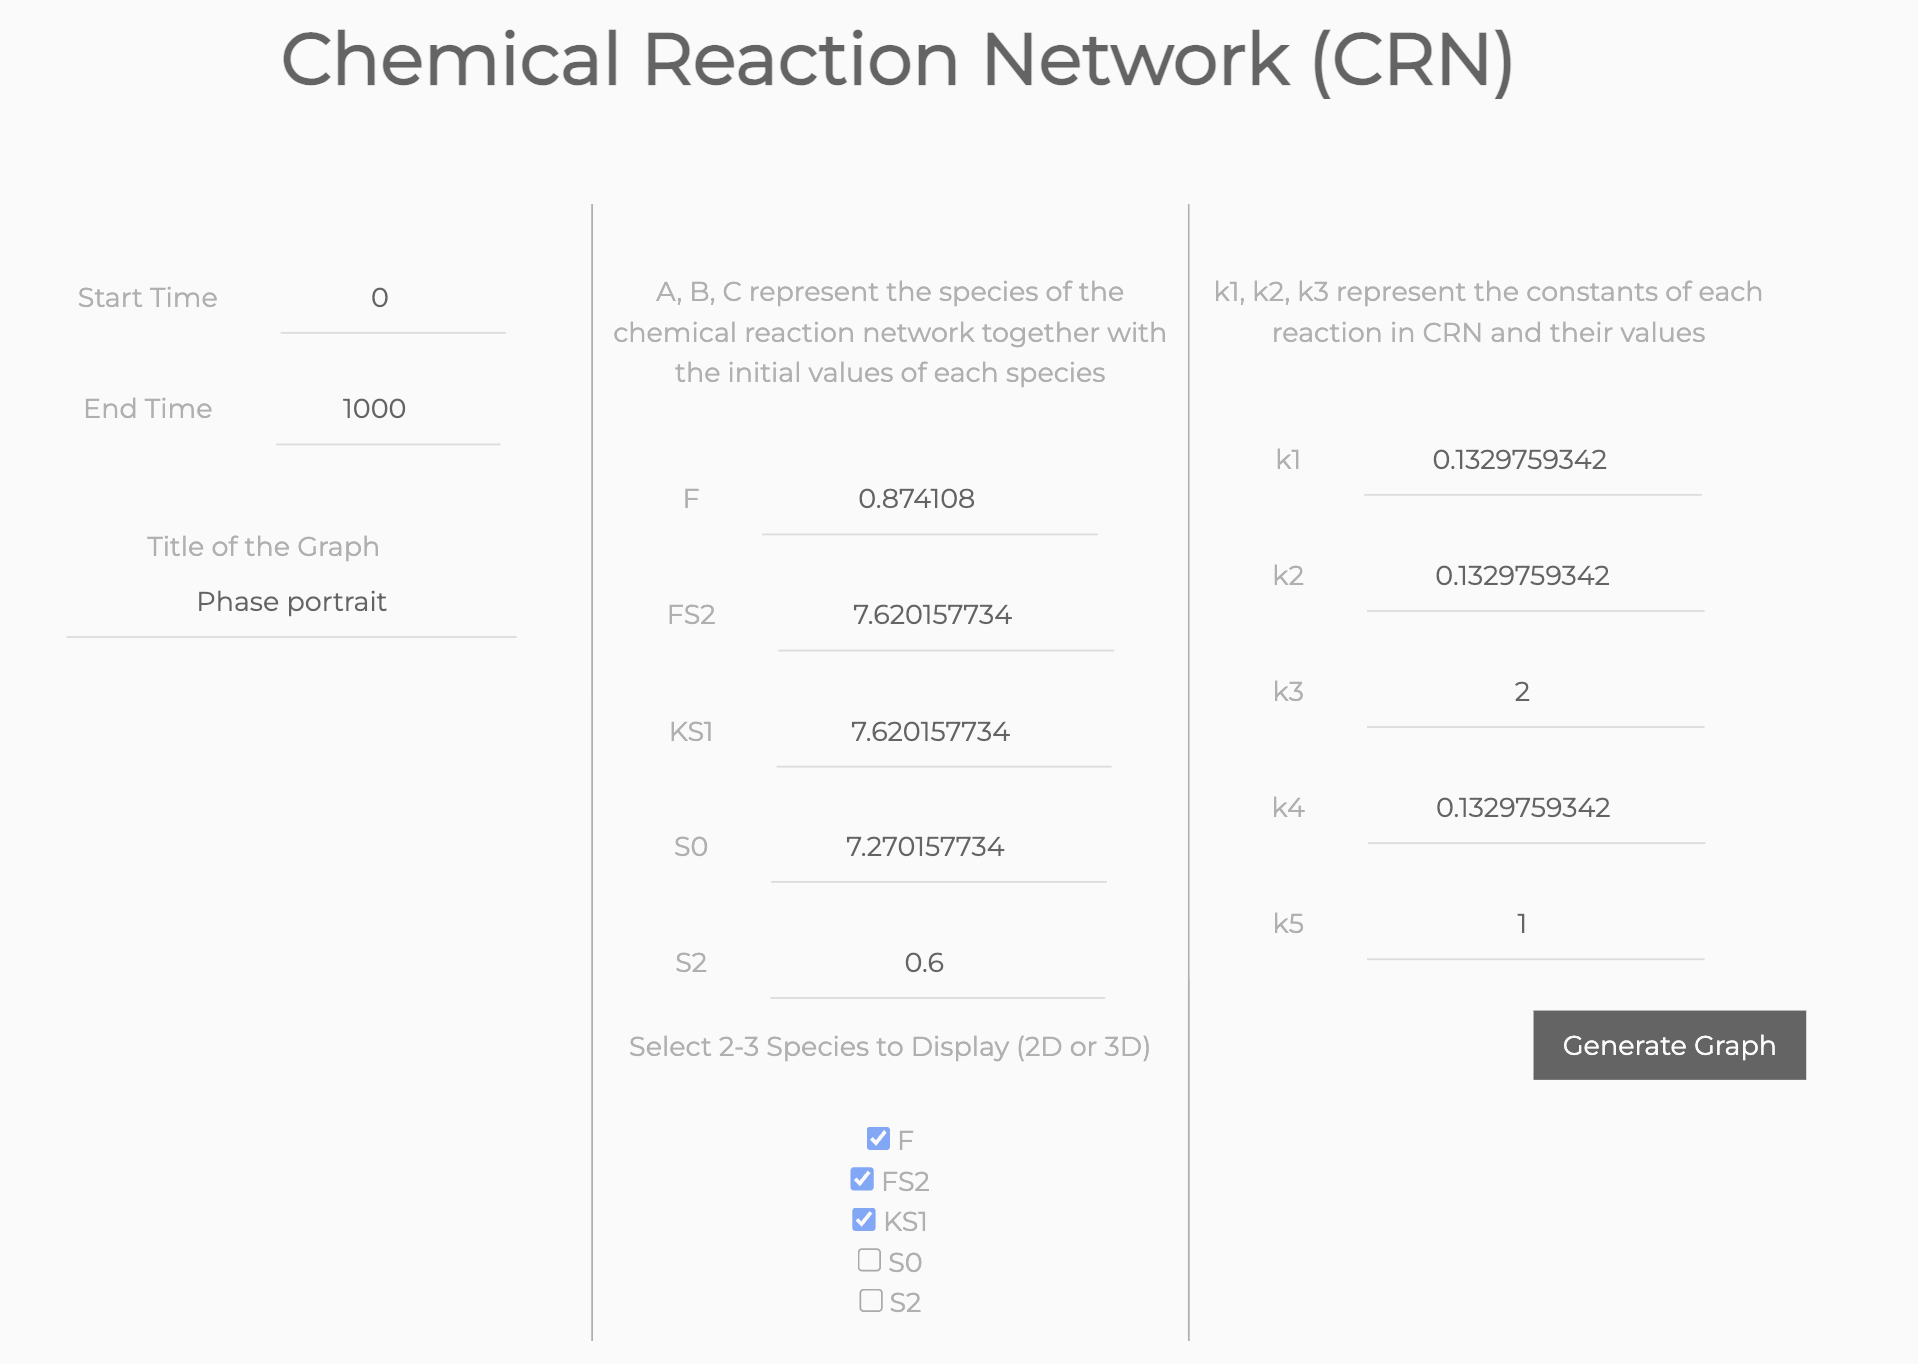
\includegraphics[width=13cm]{app_photos/3dphase-portait-input.png}\\
\].

Yielding the picture:

\[
	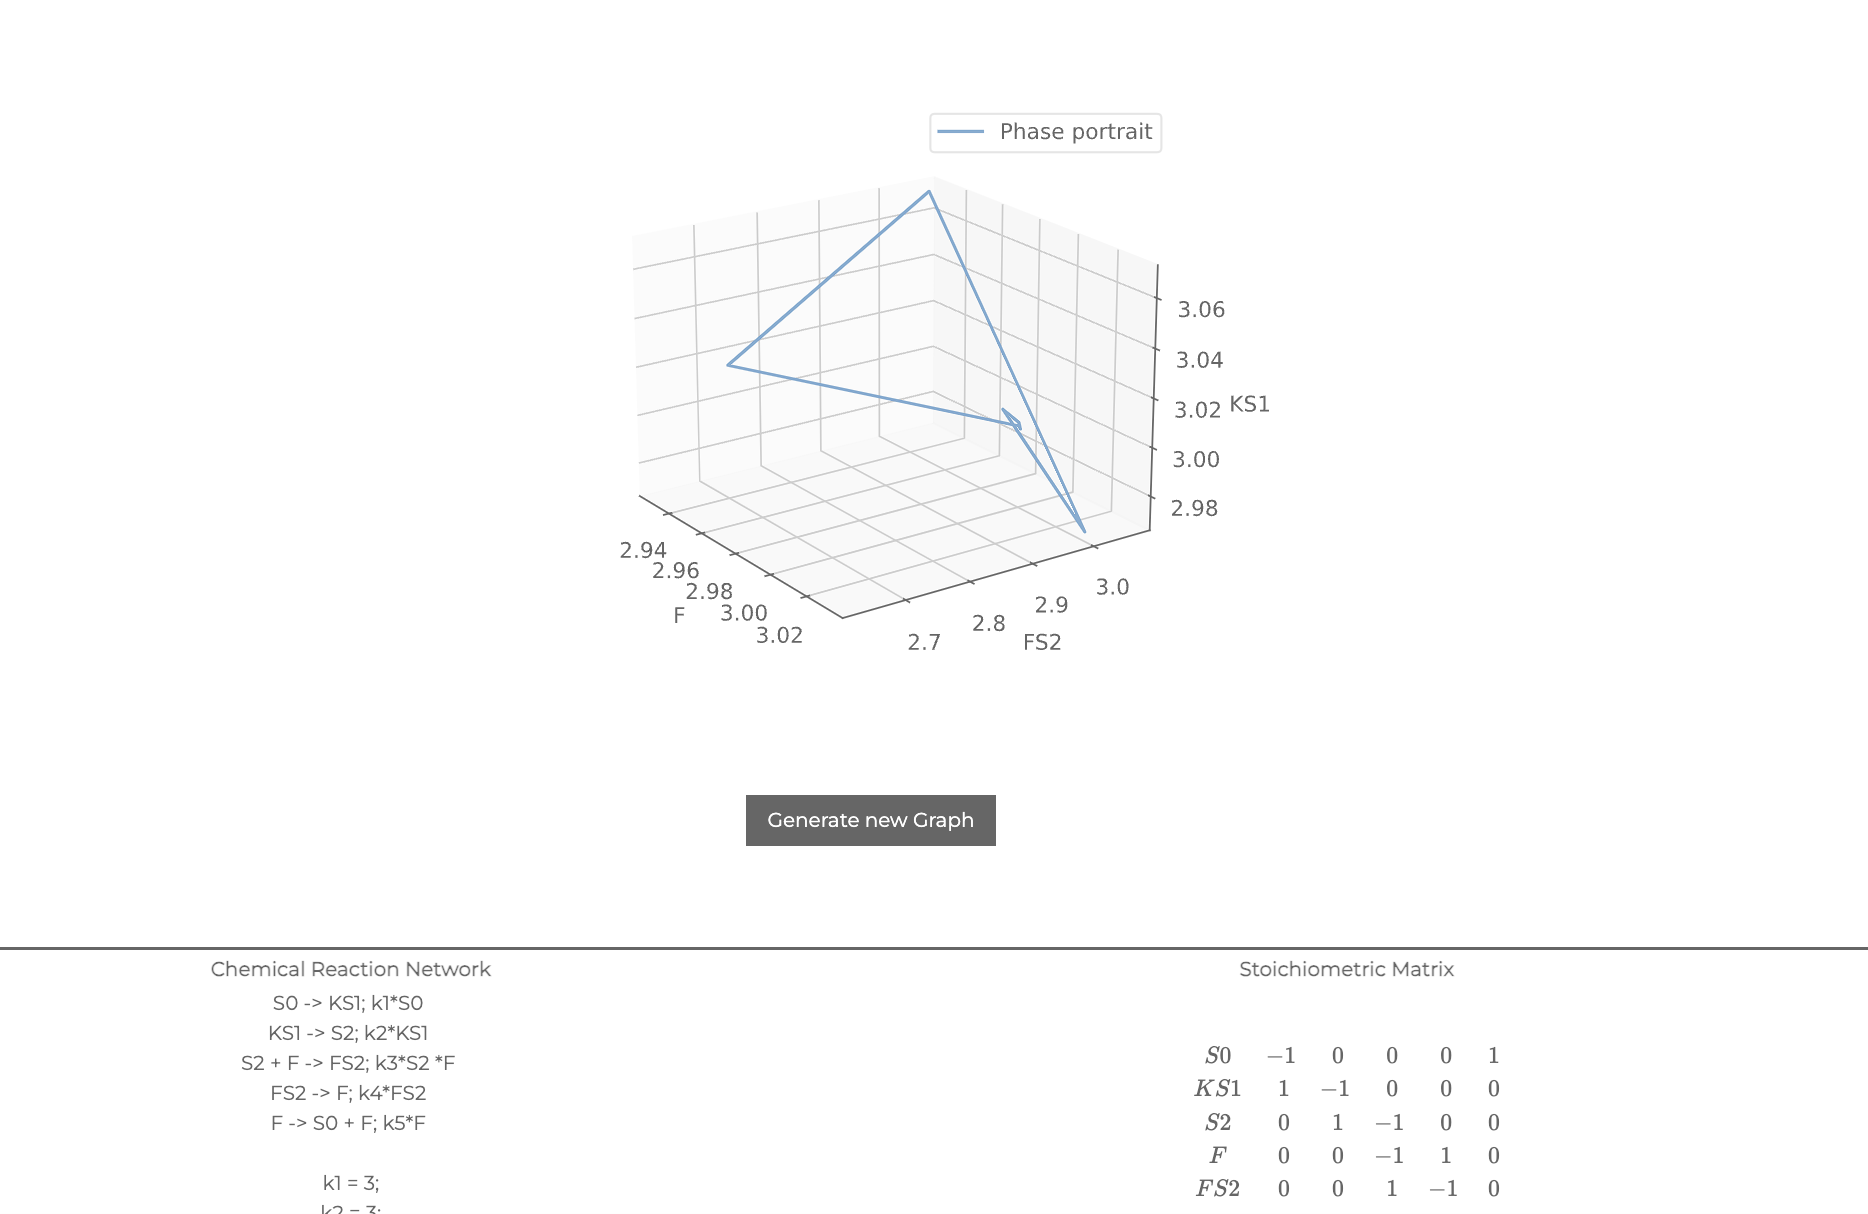
\includegraphics[width=13cm]{app_photos/3D phase portrait.png}\\
\].

Yes, it looks kind of jaggedy right now, but an extra precision-metric would come in handy.
